% SETUP
\documentclass[11pt]{article}
\linespread{1.25}
\usepackage[utf8]{inputenc}
\usepackage{graphicx, amsmath, array, graphics, amssymb, epsfig, psfrag, geometry, alltt, subfiles, blindtext, pdfpages}
\usepackage[export]{adjustbox}
\usepackage{fancyhdr}
\usepackage{array}
\usepackage{hyperref}

%%%%%%%%%%%%%%  code listing
\usepackage{listings}
\usepackage{color} %red, green, blue, yellow, cyan, magenta, black, white
\definecolor{mygreen}{RGB}{2,94,33} % color values Red, Green, Blue
\definecolor{mylilas}{RGB}{170,55,241}

\lstset{language=Matlab,%
    %basicstyle=\color{red},
    breaklines=true,%
    morekeywords={matlab2tikz},
    keywordstyle=\color{blue},%
    morekeywords=[2]{1}, keywordstyle=[2]{\color{black}},
    identifierstyle=\color{black},%
    stringstyle=\color{mylilas},
    commentstyle=\color{mygreen},%
    showstringspaces=false,%without this there will be a symbol in the places where there is a space
    numbers=left,%
    numberstyle={\tiny \color{black}},% size of the numbers
    numbersep=9pt, % this defines how far the numbers are from the text
    emph=[1]{for,end,break},emphstyle=[1]\color{black}, %some words to emphasise
    %emph=[2]{word1,word2}, emphstyle=[2]{style},    
}

\geometry{a4paper, top = 20mm, bottom = 20mm, left = 15mm, right = 15mm}

% Headers
\pagestyle{fancy}
\fancyhf{}
\chead{ELEN90064 Advanced Control Systems - Workshop 2 Report}
\cfoot{\thepage}

\begin{document}
% Cover Sheet
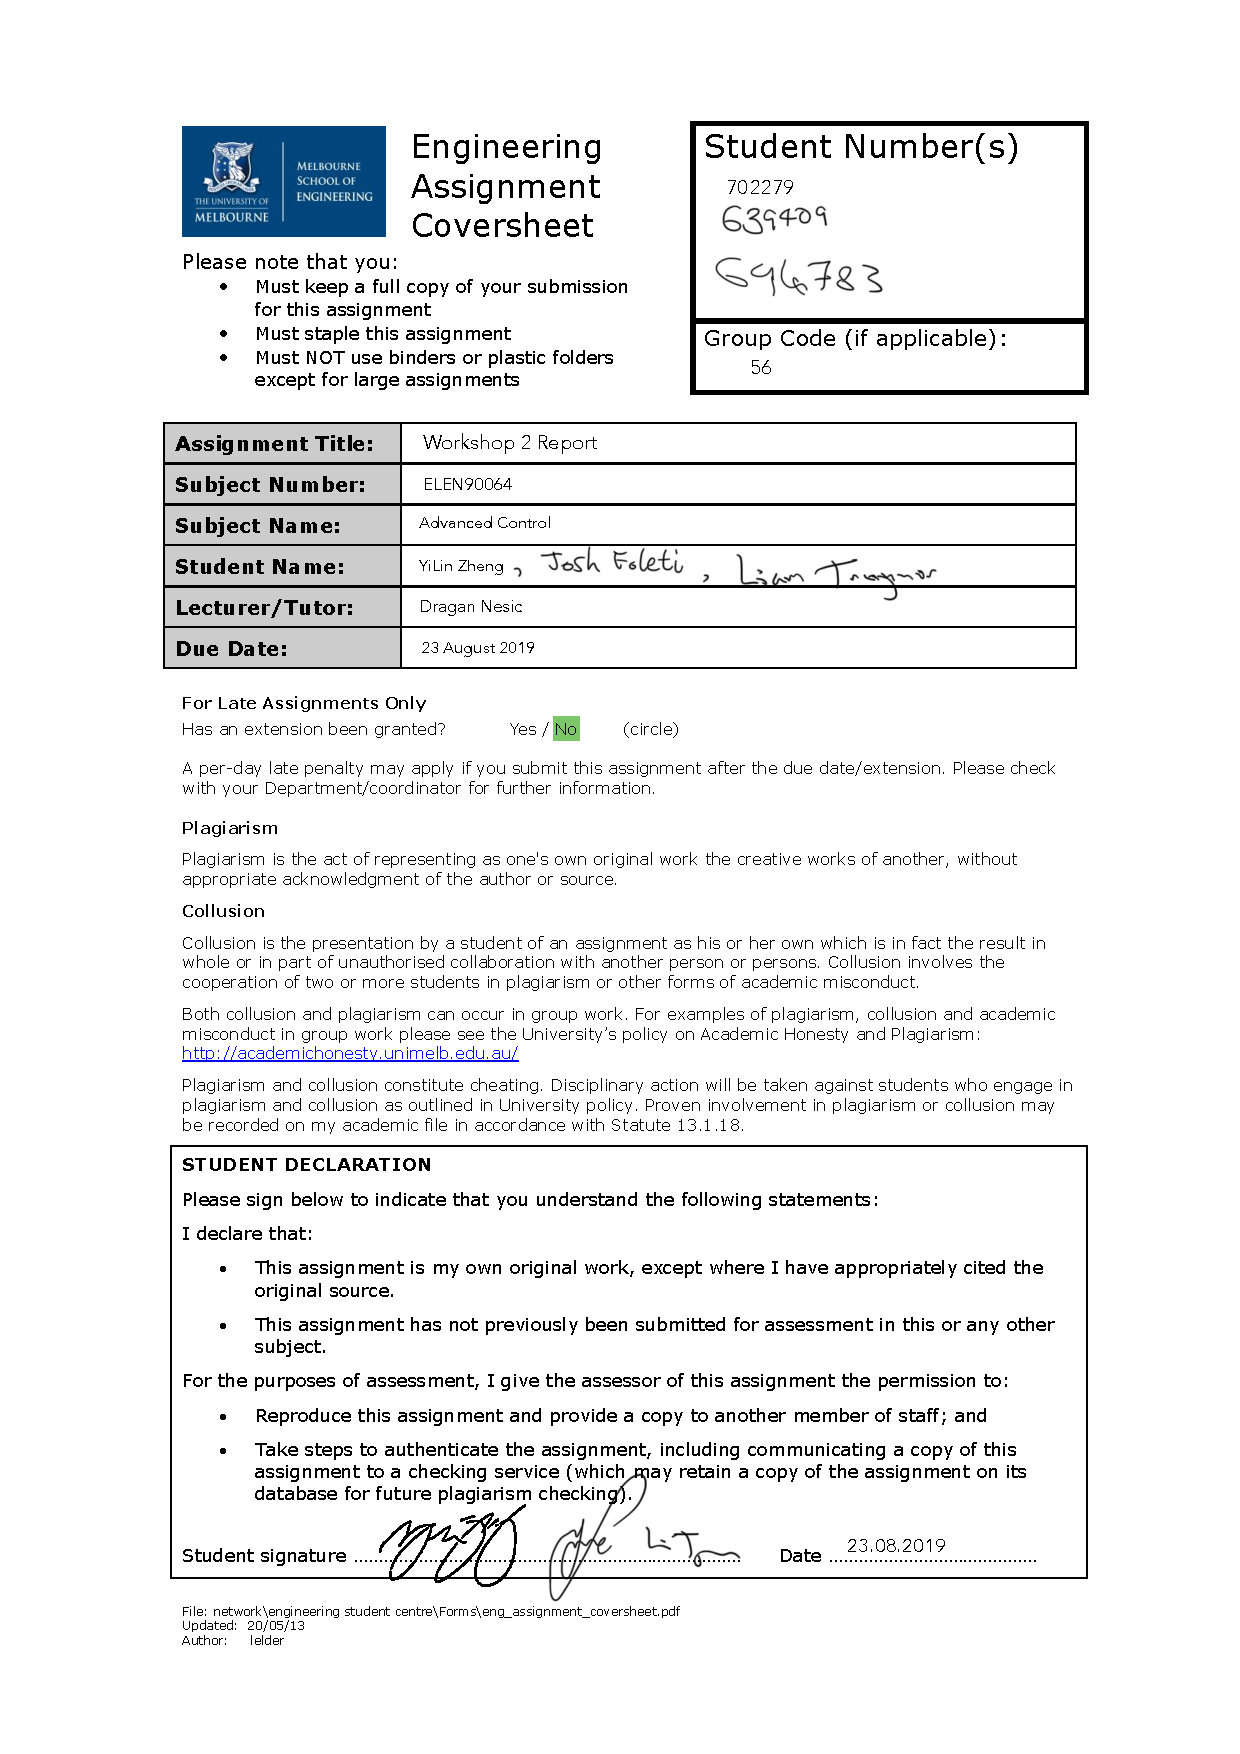
\includepdf{EngCSW2.pdf}
\clearpage
\setcounter{page}{1}

% Title
\begin{center}
\textbf{\Large{Modelling and PID Control for 1 DOF Configuration}}\\
Group 56: Josh Foleti [639409], Liam Traynor [694783], YiLin Inez Zheng [702279], \\
Workshop: Friday 1:00pm - 3:00pm Luis, Due: 23/08/19  
\end{center}

%%%%%%%%%%%%% BEGIN INTRODUCTION %%%%%%%%%%%%%%%%%
\section{Introduction}
The main objective in this workshop is to design a continuous time controller based on a continuous time 1DOF model of the Quanser Aero. Our controller must ensure the system operates at critical damping and has a settling time of 2\% in 10 seconds given a reference step input. 

% Some description about what we did, steps for analysis and design
\subsection{Method}
\begin{enumerate}
    \item %1
    Experimented with the Quanser Aero system to determine basic parameters and coefficients. 
    \item %2
    Theoretically derived the system's transfer function based on a linearised model. 
    \item %3
    Design and simulate a PID controller using Simulink.
    \item %4
    Implement the PID controller and tune it on the Quanser Aero to reach critical damping.
\end{enumerate}

%%%%%%%%%%%% BEGIN SYSTEM MODELLING SECTION %%%%%%%%%%%%%%%%
\section{System Modelling}
Based on the system mechanics and circuitry, the single axes (1DOF) system can be described by Eq.\ref{Eq.1}, where $V = V_1 - V_0$ the voltage difference between motor 1 and motor 0. 
\begin{equation}\label{Eq.1}
    J_p \ddot{\theta} = -M_b g D_m \sin \theta - b_p \dot{\theta} + K_t D_t V
\end{equation}

%EMPIRICAL DATA
\subsection{Parameters and Coefficients}
We are given the values of the aero body mass $M_b = 1.15kg$, the thrust displacement $D_t = 0.158m$ and center of mass displacement $D_m = 0.0071m$ in the Quanser Aero System Identification document. We also took the value of gravitational acceleration as $g = 9.81m s^{-2}$.\\
To obtain the rest of the system's parameters, we focused on the '0' side of the Quanser Aero (1 DOF), to which motor we gave a 24V step input for 10 seconds. The subsequent free oscillation period of 30 seconds was also captured. Measurements of the 1) Tachometer angle, 2) Motor current and 3) Motor angular speed can be seen in Figure \ref{fig:W2_emp_data}a).
\begin{figure}[ht!]
    \centering
    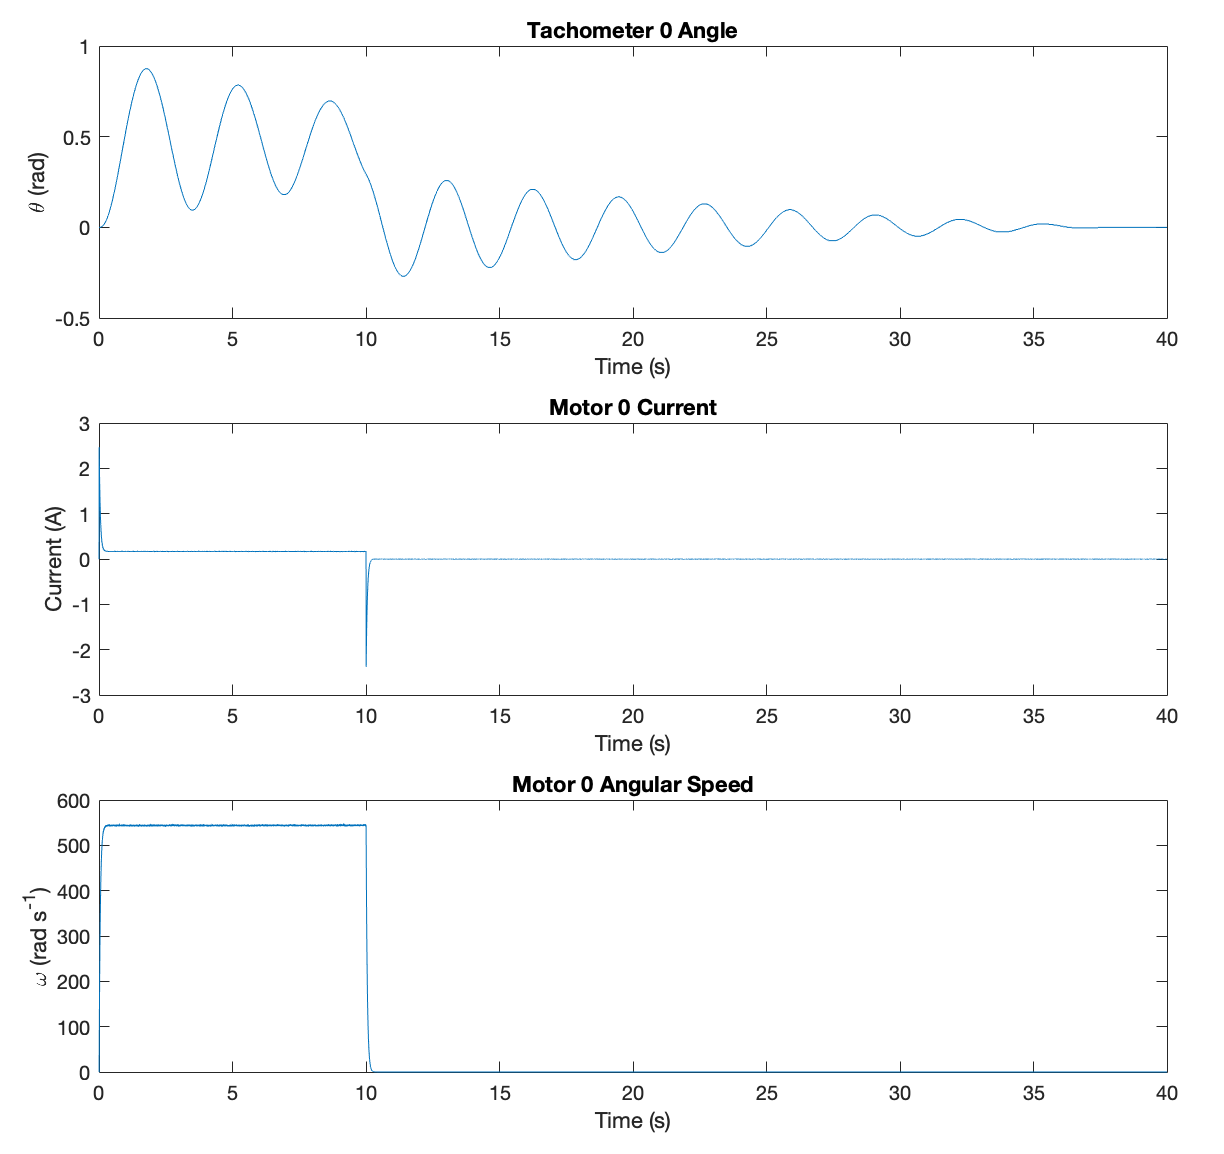
\includegraphics[scale = 0.35]{W2Empirical.png}
    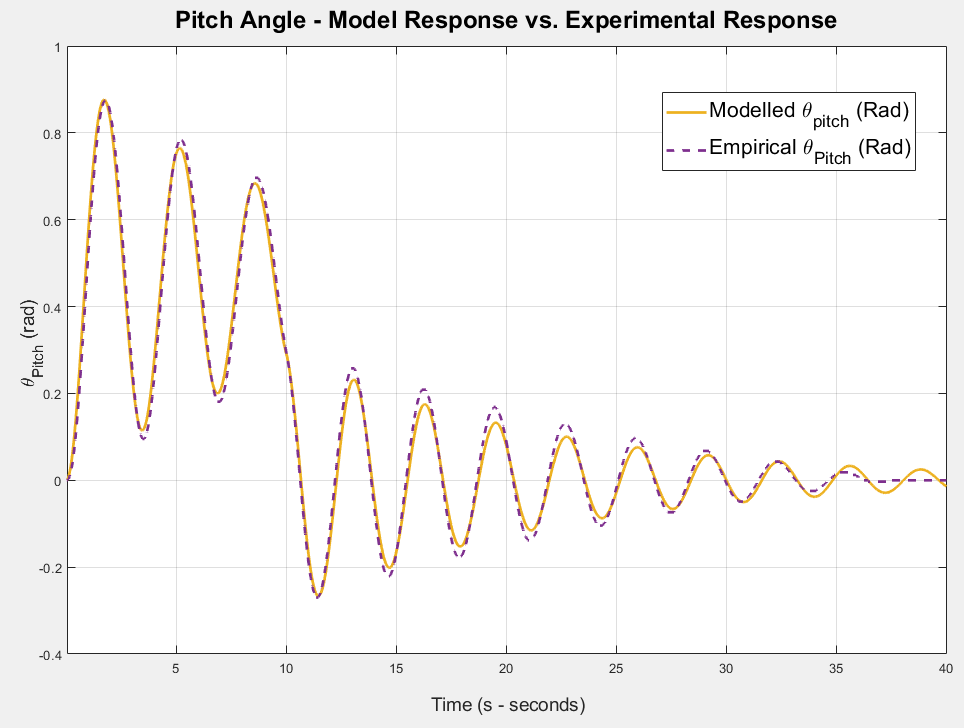
\includegraphics[scale = 0.35]{WS2_10sData2.PNG} %W2ModelVSEmp.png
    \caption{a) Measured empirical data captured via MATLAB b) Modelled tachometer step response for a 24V 10s input with empirical parameters vs. Empirical tachometer step response}
    \label{fig:W2_emp_data}
\end{figure}
\begin{itemize}
    \item %Kt
    The tachometer stabilises at $\theta = 0.455$rad whilst being powered and we obtain the thrust constant $K_t = \frac{M_b g D_m \sin(\theta)}{V_0 D_t} = 0.0093Ns\text{rad}^{-1}$
    \item %Jp
    Through finding the natural frequency $w_n = 1.9543$Hz, using the average time between periods in free oscillation, we determine the mass moment of inertia $J_p = \frac{M_b g D_m}{{w_n}^2} = 0.0210kgm^2$
    \item %Dp
    The time constant $\tau_b = 5.80s$ was used to calculate the viscous damping coefficient $D_p = \frac{J_p}{\tau_b} = 0.0036kgm^2s^{-1}$
\end{itemize}
Using our empirically obtained parameters and coefficients, we implemented the model in Simulink to compare its step response with our empirical data. This came to be fairly close and only deviated towards the end of free oscillation. See this in Figure \ref{fig:W2_emp_data}b). \textit{See Appendix \ref{sim_check_emp} Figure \ref{fig:sim_check_emp} for Simulink model.}

%% LINEARISATION
\subsection{Linearisation and deriving the CLTI Transfer Function}
Using state space variables $x_1 = \theta = f$, $x_2 = \dot{\theta} = \dot{x_1}$, and $u_1 = V$ we can express the system in Eq.\ref{Eq.1} as,
\begin{align*}
    \dot{x_2} &= -\frac{M_b g D_m}{J_p}\sin x_1 - \frac{b_p}{J_p}x_2 + \frac{K_t D_t}{J_p}u_1\\
    \dot{x_1} &= x_2
\end{align*}
As these are dynamic equations, at equilibrium $\dot{x_1} = 0$ and $\dot{x_2} = 0$. This gives us equilibrium values of $\bar{x}_1 = n\pi$ (where $n = 0, 1, 2, 3$...) and $\bar{x}_2 = 0$. We also assume the input $\bar{u}_1 = 0$ at equilibrium.\\
Now, linearising equation \ref{Eq.1} we rewrite it with $x_1 = \bar{x}_1 + \delta_{x_1}$, $x_2 = \bar{x}_2 + \delta_{x_2}$ and $u_1 = \bar{u}_1 + \delta_{u_1}$.
\begin{align*}
    \dot{\delta}_{x_1} &= \delta_{x_2}\\
    \dot{\delta}_{x_2} &= l(\bar{x}_2, \bar{x}_1, \bar{u}_1) + \frac{\partial l}{\partial x_2} \Biggr|_{(\bar{x}_2, \bar{x}_1, \bar{u}_1)} \delta_{x_2} + \frac{\partial l}{\partial x_1} \Biggr|_{(\bar{x}_2, \bar{x}_1, \bar{u}_1)} \delta_{x_1} + \frac{\partial l}{\partial u_1} \Biggr|_{(\bar{x}_2, \bar{x}_1, \bar{u}_1)} \delta_{u_1}\\
    &= \frac{-b_p}{J_p}\delta_{x_2} - \frac{M_b g D_m}{J_p}\cos \bar{x}_1 \delta_{x_1} + \frac{K_t D_t}{J_p}\delta_{u_1}
\end{align*}
Substituting the equilibrium point of $ (\bar{x}_2,\bar{x}_1)=(0,0)$  we have,
\begin{align*}
    \dot{\delta}_{x_1} &= \delta_{x_2}\\
    \dot{\delta}_{x_2} &= \frac{-b_p}{J_p}\delta_{x_2} - \frac{M_b g D_m}{J_p} \delta_{x_1} + \frac{K_t D_t}{J_p}\delta_{u_1}
\end{align*}
The state matrices are therefore found to be, 
\[ 
\mathbf{A} = \begin{bmatrix}
    0 & 1\\
    - \frac{M_b g D_m}{J_p} & \frac{-b_p}{J_p}
\end{bmatrix} \hspace{1cm}
\mathbf{B} = \begin{bmatrix}
    0\\
    \frac{K_t D_t}{J_p}
\end{bmatrix} \hspace{1cm}
\mathbf{C} = \begin{bmatrix}
    1 & 0
\end{bmatrix} \hspace{1cm}
\mathbf{D} = \begin{bmatrix}
    0 & 0
\end{bmatrix}
\]
From the state matrices, we can derive the transfer function of the continuous time model.
\begin{align*}
    G(s) = \frac{Y(s)}{U(s)} &= \mathbf{C}(s\mathbf{I} - \mathbf{A})^{-1}\mathbf{B} + \mathbf{D}\\
    &= \frac{\begin{bmatrix}
    1 & 0
\end{bmatrix} \begin{bmatrix}
    \frac{-b_p}{J_p} & - 1\\
    \frac{M_b g D_m}{J_p} & 0
\end{bmatrix} \begin{bmatrix}
    0\\
    \frac{K_t D_t}{J_p}
\end{bmatrix}}{s^2 + \frac{-b_p}{J_p}s + \frac{M_b g D_m}{J_p}}\\
&= \frac{\begin{bmatrix}
    \frac{-b_p}{J_p} & - 1
\end{bmatrix} \begin{bmatrix}
    0\\
    \frac{K_t D_t}{J_p}
\end{bmatrix}}{s^2 + \frac{-b_p}{J_p}s + \frac{M_b g D_m}{J_p}}\end{align*}
\begin{equation}\label{eq:TF}
\Rightarrow G(s) = 
    \frac{\frac{K_t D_t}{J_p}}{s^2 + \frac{-b_p}{J_p}s + \frac{M_b g D_m}{J_p}}
\end{equation}
Substituting the empirical parameter values using MATLAB we have,
\begin{figure}[ht!]
    \centering
    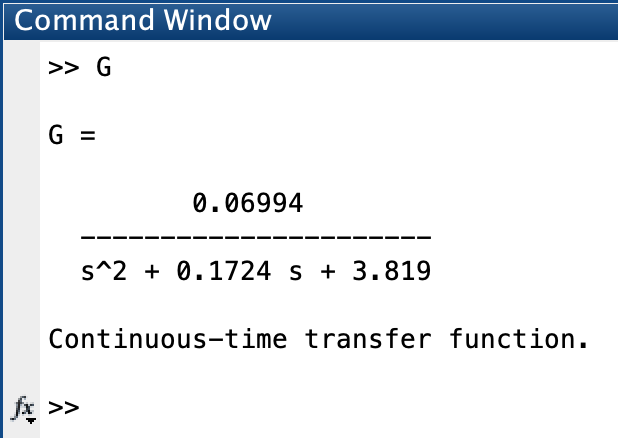
\includegraphics[scale=0.5]{W2G.png}
    \caption{MATLAB output of the linearised transfer function}
    \label{fig:W2G}
\end{figure}

\subsection{PID Controller Design}
Using our transfer function, we analysed the system in terms of its bode and root locus plots shown in Figure \ref{fig:G_bode_rlocus}. The natural frequency peak in the Bode at 1.95Hz corresponds to our empirical measurement. The root locus plot shows the two complex conjugate poles in the left half plane (stable system) but indicates overshoot, which increases as $K$ gets larger. 
\begin{figure}[ht!]
    \centering
    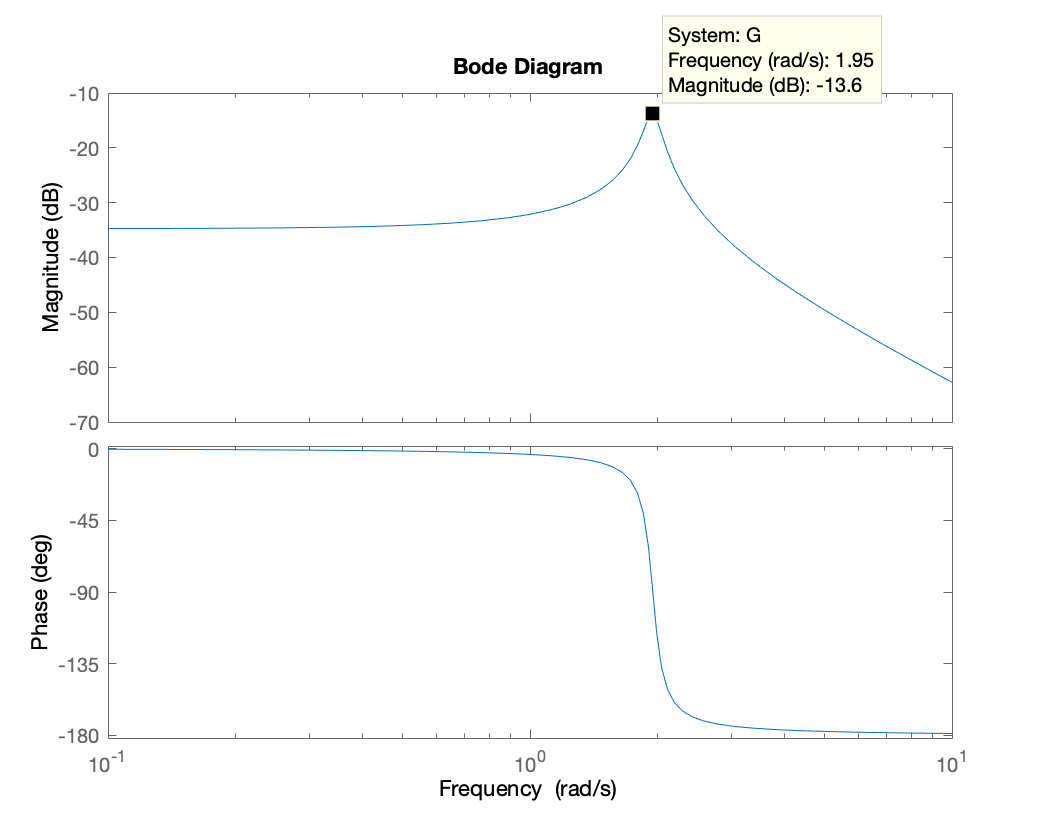
\includegraphics[scale=0.44]{W2GBode.png}
    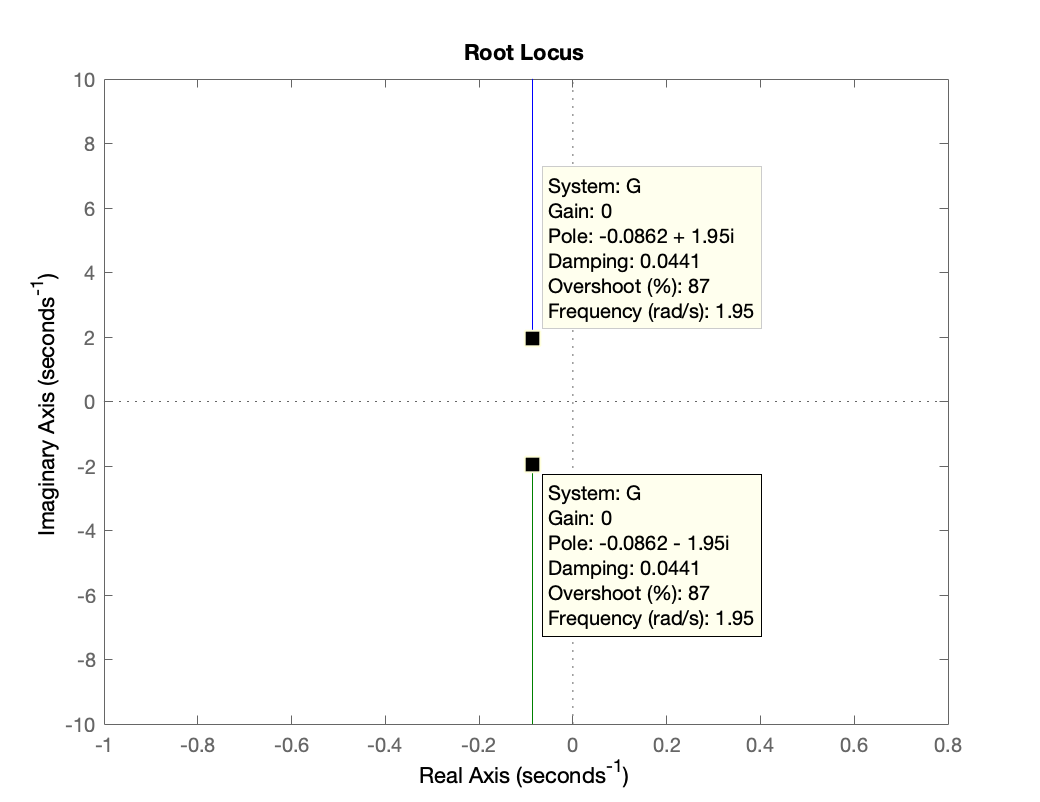
\includegraphics[scale=0.44]{W2Grlocus.png}
    \caption{a) Bode plot of $G(s)$ b) Root locus plot of $G(s)$}
    \label{fig:G_bode_rlocus}
\end{figure}

To design a PID controller, we consider that the closed loop unity feedback system has a second order transfer function of the following form, where $\omega_n$ is the natural frequency and $\zeta$ is the damping ratio.
\begin{equation}\label{eq:stepTF}
    \frac{Y(s)}{U(s)} = \frac{\omega_n^2}{s^2 + 2\zeta \omega_n s + \omega_n^2}
\end{equation}
The PID controller has the form,
\begin{equation}\label{eq:Cs}
    C(s) = k_p + \frac{k_i}{s} + k_d s
\end{equation}
and alongside our linear transfer function $G(s)$ when evaluating Eq.\ref{eq:TF}, the unity feedback loop characteristic equation is,
\begin{equation}\label{eq:Ls1}
    L(s) = s^3 + (0.06994k_d + 0.1724)s^2 + (0.06994k_p + 3.819)s + 0.06994k_i
\end{equation}
We can equate Eq.\ref{eq:Ls1} with a prototype third order characteristic equation $L(s) = (s - p_0)(s^2 + 2\zeta \omega_n s + \omega_n^2)$ to figure out the gain values $k_p$, $k_i$ and $k_d$. $p_0$ here indicates the position of a zero and $\omega_n$ and $\zeta$ indicate the output natural frequencies and damping ratio (shown in Eq\ref{eq:stepTF}).
\begin{align*}
    k_p &= \frac{\omega_n^2 + 2\zeta \omega_n p_0 - 3.819}{0.06994}\\
    k_i &= \frac{\omega_n^2 p_0}{0.06994}\\
    k_d &= \frac{2\zeta \omega_n + p_0 - 0.1724}{0.06994}
\end{align*}
To fulfil the design requirements of a critically damped system, the damping ratio is set to $\zeta = 1$. For a 2\% settling time of 10s we used $\omega_n = 1.95$, our empirical value. The zero $p_0 = 1$, when we simulated the system to get the most optimal critically damped response. Our final PID gain values were,
\begin{align*}
    k_p &= 55.89\\
    k_i &= 54.61\\
    k_d &= 67.72
\end{align*}
The simulated step response is shown in Figure \ref{fig:W2Step} below. 
\textit{See Appendix \ref{sim_step} Figure \ref{fig:sim_step} for Simulink model.}
\begin{figure}[ht!]
    \centering
    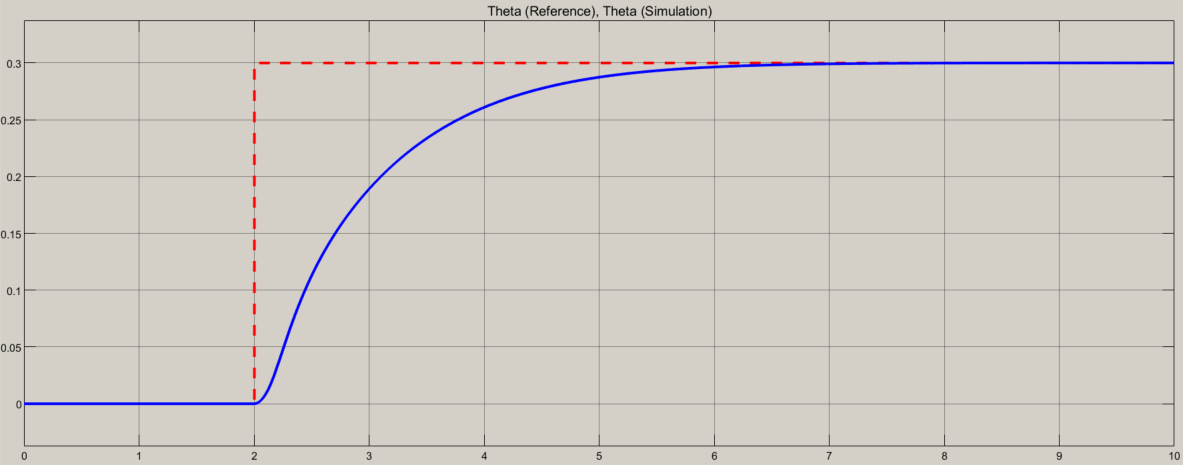
\includegraphics[scale=0.5]{WS2_Fig4_B.PNG} % Replace. W2Step.png
    \caption{Simulated step response of the close loop unity feedback system with calculated PID gain values}
    \label{fig:W2Step}
\end{figure}

%%%%%%%%%%%% BEGIN IMPLEMENTATION SECTION %%%%%%%%%%%%%%%%
\section{Implementation and Testing}
Using the $k_p$, $k_i$ and $k_d$ variables determined in the linearised model, the PID controller was implemented in Quanser Aero. Further tunings were then applied in order to meet the required specifications of critical damping and a settling time of 2\% in 10 seconds.

\subsection{Testing the model based PID design on the Quanser Aero}
%Describe drop in model compared to overshoot in Quanser.
Both the model step response and empirical Quanser Aero step response is shown in Figure \ref{fig:W2UFStep} below.
\begin{figure}[ht!]
    \centering
    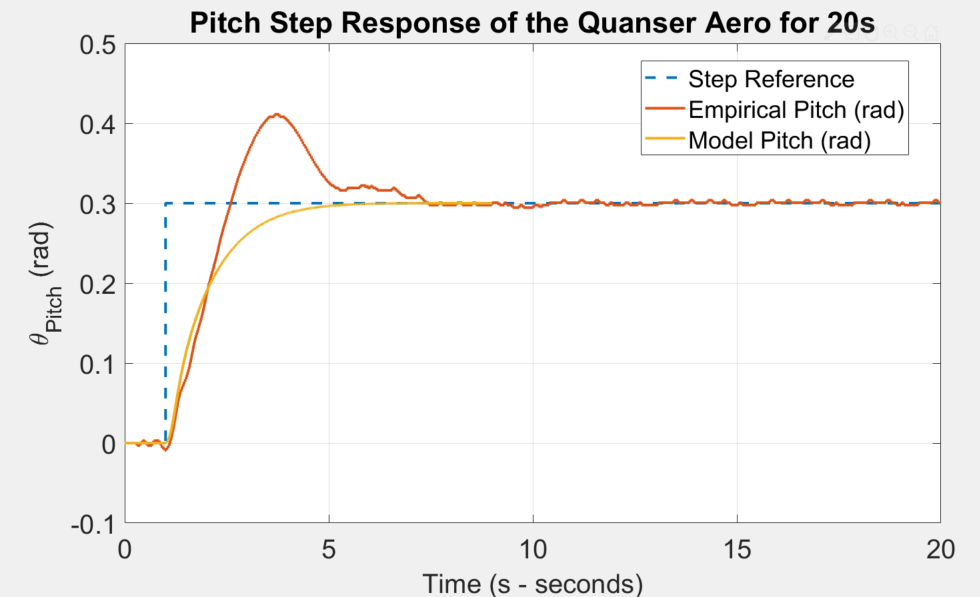
\includegraphics[scale=0.5]{WS2_PID_Test.PNG}  %  W2PIDStep.png
    \caption{Designed PID Controller Step Response}
    \label{fig:W2UFStep}
\end{figure}

 As evident, there is a large discrepancy in responses in the first 10 seconds, with the model response exhibiting expected characteristics, whereas the empirical model overshoots the steady state value by nearly 40\%. These differences can likely be contributed to the fact that the model and PID gain values are based on a second order approximation of the system in conjunction with a prototype third order characteristic equation, which may not be an accurate representation. \\
 
The above is supported by the experimental observation of heavy system vibration consistent with motor voltage saturation.\\
 
After 10 seconds the empirical response displays fluctuations in its steady state beyond the required 2\%. This, coupled with the overshoot, indicates both specification requirements were not met with the chosen PID gains. Thus further tuning is required.

\newpage
\subsection{Tuning the PID using Ziegler Nichols}
%% NOTE: Our model from the root locus suggests that no Kp will cause crossing into RHP but if this were the case, ZN would not work as Ku is when a closed loop pole touches the imaginary axis => We get constant oscillation (not growing/attenuating).
%From Figure \ref{fig:G_bode_rlocus} we can see from the root locus plot that increasing the gain will not help with the overshoot and oscillation in the system. Therefore, we chose to use the Ziegler Nichols (ZN) method to tune our PID.\\
%\colorbox{yellow}{REPLACE WITH THE FOLLOWING:}\\
Following the discussion above, it was clear a heuristic method would be preferable as a way to bypass modelling error.
Therefore, we chose to use the Ziegler Nichols (ZN) method to approximate a sensible PID controller and fine tune our PID
parameters by incremental adjustment.\\

\begin{figure}[ht!]
    \centering
    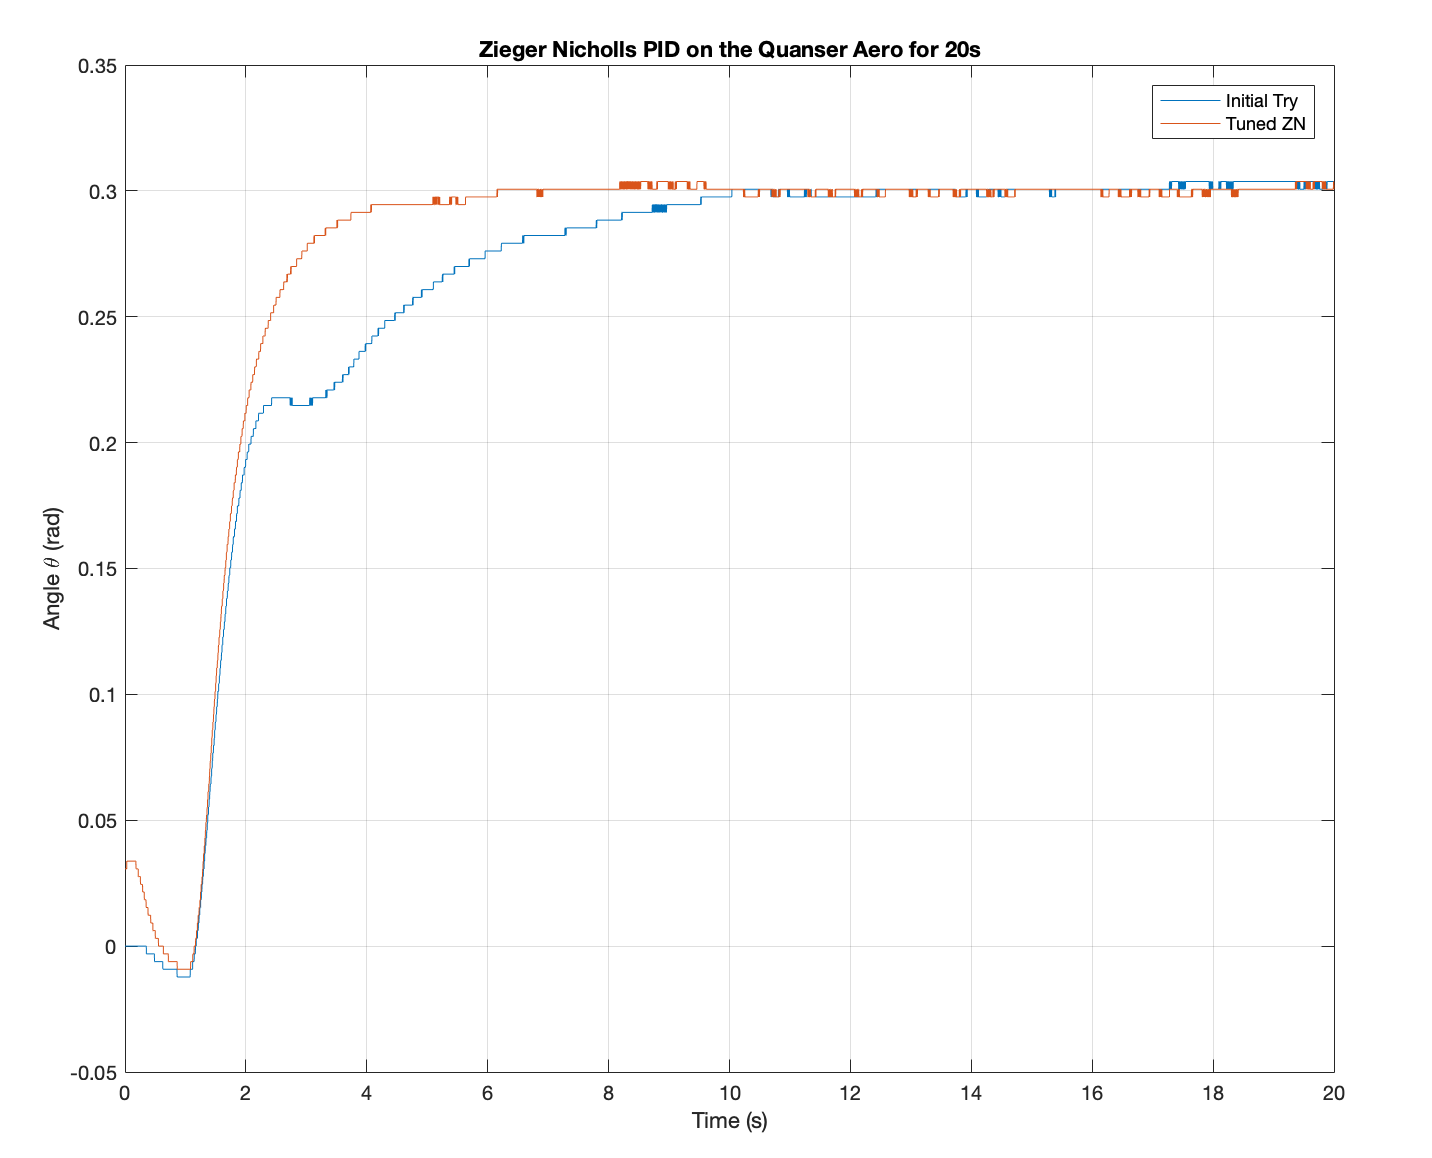
\includegraphics[scale=0.45]{W2ZNStep.png}
    \caption{Ziegler Nichols tuned PID Controller Step Response}
    \label{fig:W2ZNStep}
\end{figure}


We used the 'no overshoot' control type of the Ziegler Nichols method. As seen in Figure 6, with this primitive form, the overshoot has receded.\\

The Ziegler Nichols method produces values for the three PID parameters $k_p$, $k_i$, and $k_d$ given measurement of two
experimental parameters: the ultimate gain $K_{u}$ and oscillation period $T_{u}$.\\

With $k_{i}$ and $k_{d}$ = 0, $k_{p}$ is increased (from zero) until it reaches the ultimate gain 
$K_{u}$, at which the output of the control loop has stable and consistent oscillations of period $T_{u}$.\\

With $K_{u}$ = 20 and $T_{u}$ $\approx$ 2.453 seconds, the PID gains follow:
\begin{align*}
    k_p = \frac{K_u}{5} = 4, \hspace{1cm} k_i = \frac{\frac{2}{5}K_u}{T_u} \approx 3.26, \hspace{1cm} k_d = \frac{K_u T_u}{15} \approx 3.27
\end{align*}

These initial PID gains gave a sluggish response seen in Figure \ref{fig:W2ZNStep}.
Incrementally increasing $K_{p}$ reduced the reference gap between two and ten seconds without perturbing the steady state.\\

\colorbox{yellow}{NOTE:}
The provided Simulink Model used to drive the Quanser Aero has a "Motor Division" gain block (=7) before splitting voltage lines for Motor0 and Motor1. Considering both motors, the effective gain from the controller output is 14. Thus, the heuristic method finds PID gains that are 14 times lower than expected had the Motor Division Scheme not been included.

\newpage
\subsubsection{Tuning a square wave}
Square waves show the system's response in terms of both rise and fall.
To fine tune our critical response we observed that the tuned ZN seen in Figure \ref{fig:W2ZNSquare}
was reluctant to settle on the reference.\\

Increasing $k_p$ introduced steady-state oscillation as the small error signal would experience a
proportional gain which caused the system to overshoot. Thus, $k_i$ was increased incrementally such
that the system would reduce this error signal more slowly, as opposed to fast responses seen with proportional control.

\begin{figure}[ht!]
    \centering
    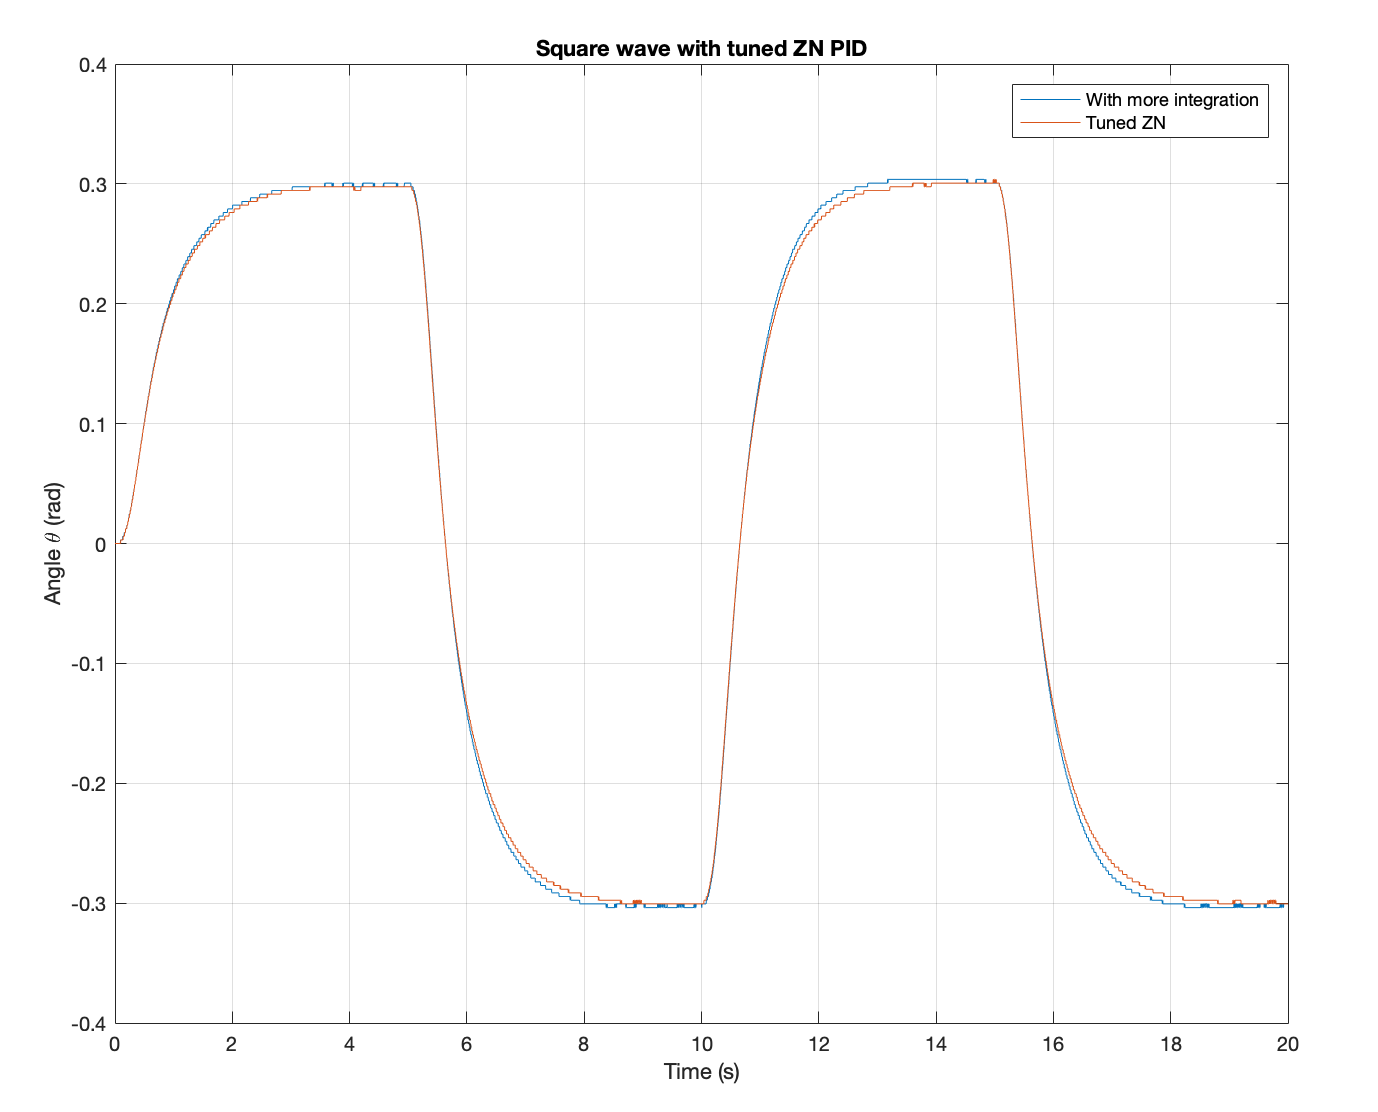
\includegraphics[scale=0.5]{W2ZNSquare.png}
    \caption{Tuning PID controller with more integration}
    \label{fig:W2ZNSquare}
\end{figure}

\newpage
\subsection{Final PID Controller}
In our most optimal configuration, the ultimate gain and subsequent PID gains were derived as above. The integral gain was then manually increased incrementally until about 10\% above its original value to $k_i = 3.5874$. The final closed loop step response with this PID controller is given below in Figure \ref{fig:W2FinalPID}. As evident, the response is critically damped and the 2\% settling time is reached within 10 seconds. Thus specifications were met.
\begin{figure}[ht!]
    \centering
    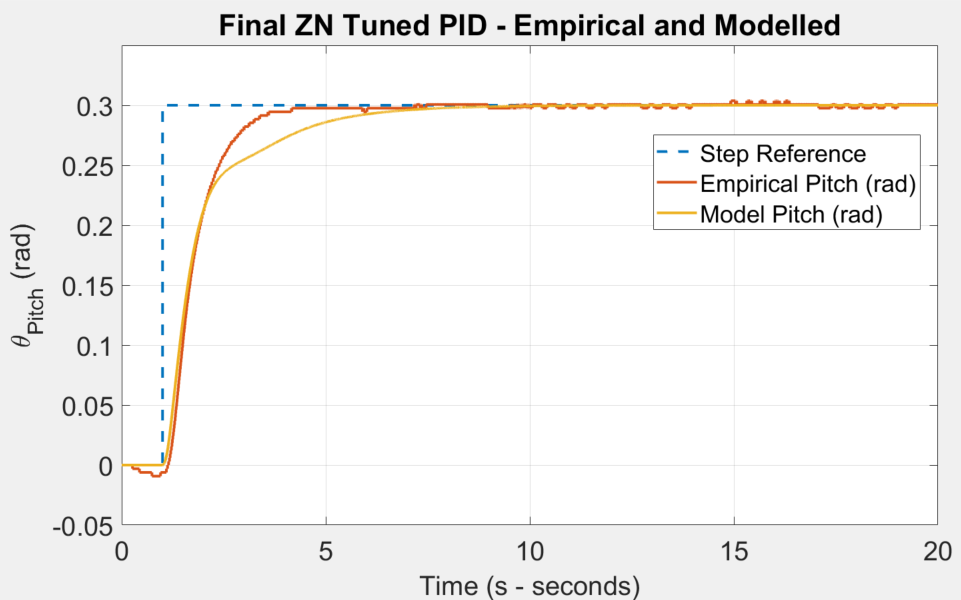
\includegraphics[scale=0.4]{WS2_Final_ZN_B.PNG} % W2FinalPID.png
    \caption{Final implemented PID}
    \label{fig:W2FinalPID}
\end{figure}

As can be seen during the transient responses (between two and five seconds) in Figure \ref{fig:W2UFStep} and Figure \ref{fig:W2FinalPID} the empirical response tends to overshoot the modelled response. Thus, even though the model in Figure \ref{fig:W2UFStep} looks critically damped, the empirical response overshoots the reference. This is most likely due to modelling error of the physical system.

%%%%%%%%%%%% BEGIN CONCLUSION %%%%%%%%%%%%%%%%
\section{Conclusions}
In this workshop, the system parameters of the Quanser Aero were derived based on the 1DOF configuration. The resulting empirical parameters were then validated with the actual system via a Simulink model, before being utilised in conjunction with a second order approximation of the closed loop system to develop a PID controller. This controller was designed such that the step response of the closed loop system was critically damped with a 2\% settling time of 10 seconds. \\

Once these specifications were met in the simulation model, the controller was implemented on Quanser Aero. Large discrepancies were found between the simulation model and the empirical model due to the simplification of the model to a second degree system as well as the physical dynamics intrinsic to the Quanser Aero. In the empirical model, system requirements were not met so further controller tuning was required. \\

Finally, these PID tuning techniques were tested and applied, specifically Ziegler Nichols. Using the `no overshoot' method and making final adjustments to the integral gain, the final closed loop step response was critically damped and reached a 2\% settling time within 5 seconds - well within the given requirements of 10 seconds.

\newpage
\section{Appendix}
\subsection{Simulink Model for checking Empirical Parameters}\label{sim_check_emp}
\begin{figure}[ht!]
    \centering
    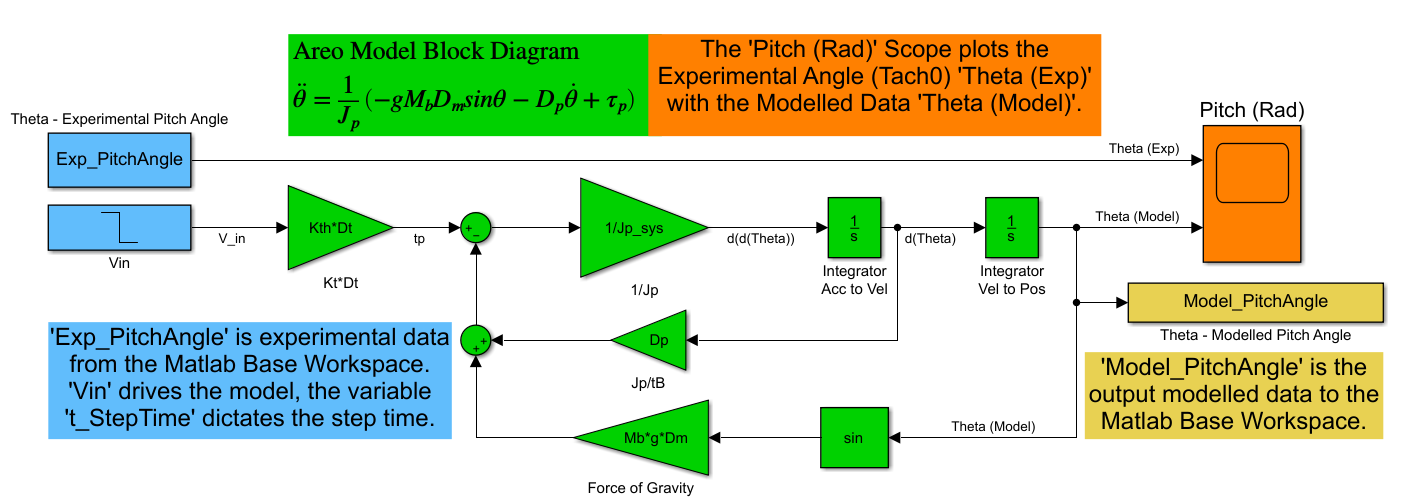
\includegraphics[scale=0.5]{WS2_SimModel.PNG} % W2sim_check_emp.png
    \caption{Simulink model for the Quanser Aero using empirical parameters}
    \label{fig:sim_check_emp}
\end{figure}
\subsection{Simulink Model for Step Response}\label{sim_step}
\begin{figure}[ht!]
    \centering
    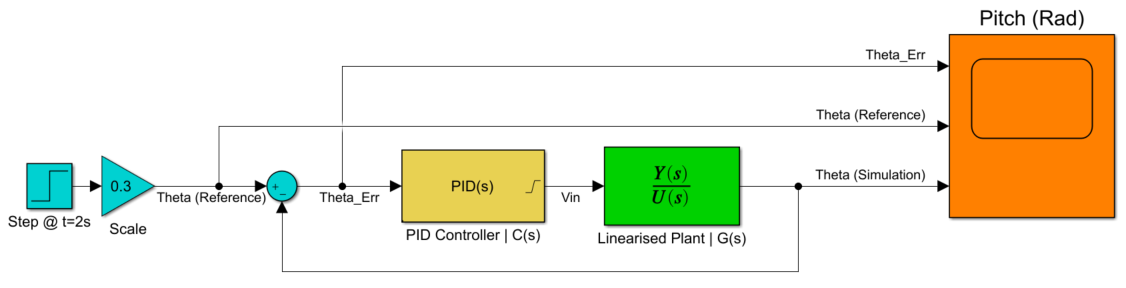
\includegraphics[scale=0.5]{WS2_SimModel_B.PNG}   % Replace: W2PIDSim.png
    \caption{Simulink model for the PID close loop unity feedback Step Response}
    \label{fig:sim_step}
\end{figure}

\subsection{MATLAB Code for Empirical Modelling}
\begin{lstlisting}[frame=single]
%% Plotting experimental data
load('matlab_exp_values.mat');

figure(1);
set(gcf,'color','w');
subplot(3,1,1);
plot(Angle_Tach0_Rad.time, Angle_Tach0_Rad.signals.values);
title('Tachometer 0 Angle');
xlabel('Time (s)')
ylabel('\theta (rad)')
subplot(3,1,2);
plot(Current_M0.time, Current_M0.signals.values);
title('Motor 0 Current')
xlabel('Time (s)')
ylabel('Current (A)')
subplot(3,1,3);
plot(Speed_M0_RadpS.time, Speed_M0_RadpS.signals.values);
title('Motor 0 Angular Speed');
xlabel('Time (s)')
ylabel('\omega (rad s^{-1})')

%% Natural Frequency wn
% Found time intervals (ts) where peaks occured
% Now calculating average time per cycle to calculate natural frequency
diff = [];
for n = 1:length(ts)-1
    diff(n) = ts(n+1)-ts(n);
end
avg_ts = mean(diff);
wn = 1/avg_ts;

run('ParametersScript.m');

%% Modelling the Quanser Aero
% Run Simulink model with the above parameters
run('W2_model.slx');

% Plotting model outcome against original signal
figure(2);
set(gcf,'color','w');
plot(model_response.time, model_response.signals.values);
hold on
plot(Angle_Tach0_Rad.time, Angle_Tach0_Rad.signals.values);
title('Model response vs. Empirical response')
xlabel('Time (s)')
ylabel('\theta (rad)')
legend('Model simulated Tachometer 0','Empirical Tachometer 0')
\end{lstlisting}

\subsection{MATLAB Code for \texttt{ParametersScript.m}}
\begin{lstlisting}[frame=single]
% System model parameters
% You need to experimentally identify these parameters
%
g = 9.81;
Mb = 1.15;
Dt = 0.158;
Dm = 0.0071;
%
% Calculate thrust constant
V_in = 24; % Volts
theta_ss = 0.455; % Radians
Kth = Mb*g*Dm*sin(theta_ss)/(V_in*Dt);
%
% Calculate moment of inertia
avg_ts = 3.215;
w_n = 2*pi/avg_ts;
Jp_sys = Mb*Dm*g/(w_n^2);
%
% Calculate the viscous damping coefficient
tau_b = 5.8; % seconds
Dp = Jp_sys/tau_b;

%% Model

A = [0 1; -Mb*g*Dm/Jp_sys -Dp/Jp_sys];
B = [0; Kth*Dt/Jp_sys];
C = [1 0];
D = [0];
[G_num, G_den] = ss2tf(A,B,C,D);

% G_num = [ 0 0 0.0699 ] // G_den = [ 1.0000 0.1724 3.8194 ]
G = tf(G_num, G_den);
%T = feedback(G,1);
\end{lstlisting}

\subsection{MATLAB Code for Controller PID}
\begin{lstlisting}[frame=single]
figure(1);
set(gcf,'color','w');
bode(G);
figure(2);
set(gcf,'color','w');
rlocus(G);

%% 2.2 Calculate PID Gains.
% Controller calculations here

a = G_num(3);   b = G_den(2);   c = G_den(3);
p0 = 1;         DampRatio = 1;  % Critically Damped.
kd = (2*DampRatio*w_n + p0 - b) / a;
kp = (w_n^2 + 2*DampRatio*w_n*p0 - c) / a;
ki = (w_n^2*p0) / a;
\end{lstlisting}

\subsection{MATLAB Code for plotting our implemented controller}
\begin{lstlisting}[frame=single]
% Zieger Nicholls PID gains
Ku = 20;
Tu = 2.453;

kp = Ku/5.5;
ki = (2.2/5)*Ku/Tu;
kd = Ku*Tu/15;

%% Step Response
load('matlab_1400_2.2_p1_wn2_dr1_PIDBLOCK_step.mat')
load('ControllerStep.mat')
figure(7);
set(gcf,'color','w');
plot(angle_unity_gain.time,angle_unity_gain.signals.values);
hold on
plot(ControllerStep.time,ControllerStep.signals.values);
hold off 
grid on
title("Step response of the Quanser Aero for 20s")
xlabel("Time (s)");
ylabel("Angle \theta (rad)")
legend("Empirical Step Response","Model Step Response");

%% Zieger Nicholls
load('matlab_1400_2.2_p1_wn2_dr1_PIDBLOCK_step_ZN.mat')
figure(10);
set(gcf,'color','w');
plot(angle_unity_gain.time,angle_unity_gain.signals.values./0.3);
hold on
load('matlab_1400_2.2_p1_wn2_dr1_PIDBLOCK_step_ZN_good_5_5.mat')
plot(angle_unity_gain.time,angle_unity_gain.signals.values);
hold off 
grid on
title("Zieger Nicholls PID on the Quanser Aero for 20s")
xlabel("Time (s)");
ylabel("Angle \theta (rad)")
legend("Initial Try","Tuned ZN");

%% Square Wave Graph
load('matlab_1400_2.2_p1_wn2_dr1_PIDBLOCK_square_ZN_good_5_5_moreintegration2_1.mat')
figure(5);
set(gcf,'color','w');
plot(angle_unity_gain.time,angle_unity_gain.signals.values./0.3);
hold on
load('matlab_1400_2.2_p1_wn2_dr1_PIDBLOCK_square_ZN_good_5_5.mat')
plot(angle_unity_gain.time,angle_unity_gain.signals.values);
hold off
grid on
title("Square wave with tuned ZN PID")
xlabel("Time (s)");
ylabel("Angle \theta (rad)")
legend("With more integration","Tuned ZN")

%% Final PID
load('matlab_1400_2.2_p1_wn2_dr1_PIDBLOCK_step_ZN_good_5_5.mat')
figure(9);
set(gcf,'color','w');
plot(angle_unity_gain.time,angle_unity_gain.signals.values);
grid on
title("Step response of the Quanser Aero for 20s")
xlabel("Time (s)");
ylabel("Angle \theta (rad)")
\end{lstlisting}
\end{document}
